% Generated by paper_assets. Rebuild: python paper-artifacts/build.py fig2_geometry_discovery
% Figure drawn at the exact \textwidth; include without rescaling.
\begin{figure*}[t]
\centering
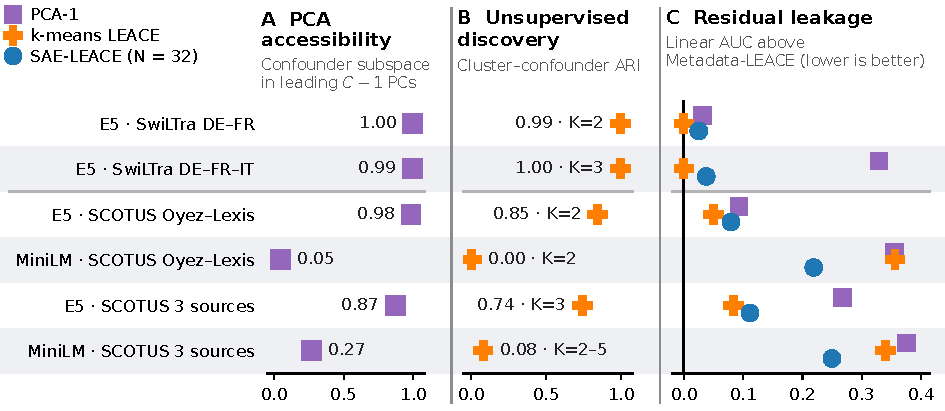
\includegraphics[width=\textwidth]{paper-artifacts/figures/fig2_geometry_discovery.pdf}
\caption{Geometry and label-free erasure. Rows are six settings (encoder $\cdot$ corpus; the line separates SwiLTra from SCOTUS). \textbf{A}~PCA accessibility: share of the supervised confounder subspace (the rank-$(C-1)$ span of the label cross-covariance, which Metadata-LEACE removes) captured by the leading $C-1$ principal components of the training embeddings. \textbf{B}~Unsupervised discovery: adjusted Rand index between the silhouette-selected $k$-means groups and the confounder classes (post hoc), with the selected $K$ (a range where seeds differ). \textbf{C}~Residual leakage: held-out linear AUC of each label-free eraser minus that of Metadata-LEACE, formed per seed (0 = the supervised reference). Points are seed means (SDs in the data files). A, B and C all use seeds 0--4: the geometry run and each setting's performance cohort, both extended from seeds 0--2 where they had only three. Leading PCs needed for 90\% capture, by row: 1: 1; 2: 2; 3: 1; 4: 22–29; 5: 2–3; 6: 17–19.}
\label{fig:geometry-discovery}
\end{figure*}
